\section{Results}\label{sec:results}

All statements below concern four models of one vendor. Model-versus-model and condition-versus-condition differences are reported with the tests described in Section~\ref{sec:stats}. All pairwise model tests are listed in Table~\ref{tab:pairs}, and the full per-genre and per-condition breakdown is in Table~\ref{tab:breakdown} (Appendix~\ref{secA2}).

\subsection{Study 1: how often the models assert text that is not there (RQ1)}\label{sec:rq1}

Table~\ref{tab:rates} summarises the outcomes over all \NImages{} synthetic images. Measured per quoted word, hallucination is rare: \HallPHaikuDesc\% of the words Haiku quotes in its descriptions are misread or fabricated, \HallPSonnetDesc\% for Sonnet, \HallPOpusDesc\% for Opus and \HallPFableDesc\% for Fable. Measured per response, which is what a blind user experiences, it is common. A description contains at least one hallucinated word in \ImgPHaikuDesc\% (Haiku), \ImgPSonnetDesc\% (Sonnet), \ImgPOpusDesc\% (Opus) and \ImgPFableDesc\% (Fable) of the images. Within this model family, the most expensive model is not the most faithful reader. Fable produces a hallucinated word in more descriptions than Sonnet (Holm-corrected McNemar $p=\SynPairSonnetFableP$) and Opus ($p=\SynPairOpusFableP$), and Haiku in more than Sonnet ($p=\SynPairHaikuSonnetP$). The other pairs do not differ reliably (Table~\ref{tab:pairs}). In \RangeImgUnh\% of the images, at least one hallucinated word is stated without any hedging in its sentence, so the listener has no cue to doubt it. Hallucination is not confined to degraded images: even for clean, fully framed images, \ImgCleanFullHaiku\% (Haiku), \ImgCleanFullSonnet\% (Sonnet) and \ImgCleanFullOpus\% (Opus) of the descriptions contain a hallucinated word. At least one wrong digit group, which can affect dates, doses, prices, phone or account numbers, appears in \ImgDigitHaiku\%, \ImgDigitSonnet\% and \ImgDigitOpus\% of the descriptions. Reading coverage is high: the models quote \RangeCov\% of the visible ground-truth words.

\begin{table}[t]
\caption{Study~1 (synthetic, \NImages{} images): text-reading outcomes per model and prompt. Token rates are percentages of all quoted (description) or transcribed (transcription) tokens; brackets give Wilson 95\% intervals. ``Responses'' is the percentage of images whose response contains at least one hallucinated (misread or fabricated) token. Coverage is the percentage of visible ground-truth tokens that the response reads correctly.}\label{tab:rates}
\footnotesize
\setlength{\tabcolsep}{3pt}
\begin{tabular*}{\textwidth}{@{\extracolsep\fill}llrlrrrlr}
\toprule
Model & Prompt & Tokens & Hallucinated \% & Misread & Fabric. & Completion & Responses \% & Cover. \\
\midrule
%TABLE:rates%
\botrule
\end{tabular*}
\end{table}

\paragraph{Image quality and framing.} Table~\ref{tab:breakdown} (Appendix~\ref{secA2}) breaks down the rates by genre, quality, framing and word category. Figures in this paper show the real-image Study~2; the corresponding Study~1 numbers are given in the tables and the text. Severe degradation is the dominant driver. For every model, both the image-level rate and the token-level rate rise from clean to severe images (e.g., Haiku \SynCHaikuSevereCleanImg{} of descriptions with a hallucination, Holm $p=\SynCHaikuSevereCleanP$; token-rate difference \SynCHaikuSevereCleanTok{} percentage points; Sonnet \SynCSonnetSevereCleanImg{}, Opus \SynCOpusSevereCleanImg{}, Fable \SynCFableSevereCleanImg{}, all $p<0.001$). Moderate blur does not raise the rate: for every model the token-rate difference from clean includes zero (Haiku \SynCHaikuBlurCleanTok, Sonnet \SynCSonnetBlurCleanTok, Opus \SynCOpusBlurCleanTok). Occlusion by a finger or glare raises the image-level rate for Haiku (\SynCHaikuOcclusionNoneImg, $p=\SynCHaikuOcclusionNoneP$) and Sonnet (\SynCSonnetOcclusionNoneImg, $p=\SynCSonnetOcclusionNoneP$), but not reliably for Opus ($p=\SynCOpusOcclusionNoneP$) or Fable ($p=\SynCFableOcclusionNoneP$). A crop by the frame edge does not raise the misreading rate (all $p=1$ after correction) but produces completions (Section~\ref{sec:completion}). Per quoted word, signage is hallucinated more often than documents for every model (token-rate differences Haiku \SynCHaikuSignageDocumentTok, Sonnet \SynCSonnetSignageDocumentTok, Opus \SynCOpusSignageDocumentTok{} percentage points). The image-level difference, however, is not significant ($p=\SynCHaikuSignageDocumentP$ for Haiku), because signage carries fewer words per image.

\paragraph{What kind of text is misread.} The category of the printed word matters as much as image quality (Table~\ref{tab:breakdown}). Common words are hallucinated at \CatWordHaiku\% (Haiku), \CatWordSonnet\% (Sonnet) and \CatWordOpus\% (Opus), and real names at similar rates. Invented names, which no language prior can predict, are misread or replaced at \CatNonceHaiku\%, \CatNonceSonnet\% and \CatNonceOpus\%. Near-word names, one letter away from a real word, are misread at \CatLureHaiku\%, \CatLureSonnet\% and \CatLureOpus\%. Digits sit in between (\CatNumHaiku\%, \CatNumSonnet\%, \CatNumOpus\%). For the near-word names, the misreading is very often the real word: \LureLexHaiku\% (Haiku), \LureLexSonnet\% (Sonnet) and \LureLexOpus\% (Opus) of the claims matched to a near-word name are the lexicalised original. Examples are \foreignlanguage{ukrainian}{«Метфермін»} read as \foreignlanguage{ukrainian}{«Метформін»}, \foreignlanguage{ukrainian}{«Добробїт»} as \foreignlanguage{ukrainian}{«Добробут»} and \foreignlanguage{ukrainian}{«Воложка»} as \foreignlanguage{ukrainian}{«Волошка»}. The near-word probe on real documents (Section~\ref{sec:probe_res}) shows the same normalisation on real pages.

\paragraph{Ukrainian orthography.} Among claims matched to invented names, \NonceUaHaiku\% (Haiku), \NonceUaSonnet\% (Sonnet) and \NonceUaOpus\% (Opus) differ from the printed form only in replacing \foreignlanguage{ukrainian}{ї, є} or \foreignlanguage{ukrainian}{ґ} by \foreignlanguage{ukrainian}{і, е} or \foreignlanguage{ukrainian}{г}, i.e., by spellings shared with Russian (e.g., \foreignlanguage{ukrainian}{«Пїжєназол»} read as \foreignlanguage{ukrainian}{«Піженазол»}). This rate is inflated by the synthetic invented names, which over-represent these letters (Section~\ref{sec:setcompare}). Across all hallucinated words in descriptions, the error taxonomy is as follows. Ukrainian-letter substitutions account for \SubUaHaiku\% (Haiku), \SubUaSonnet\% (Sonnet) and \SubUaOpus\% (Opus), digit errors for \SubDigitHaiku\%, \SubDigitSonnet\% and \SubDigitOpus\%, lexicalisations for \SubLexHaiku\%, \SubLexSonnet\% and \SubLexOpus\%, and fabrications for \SubFabHaiku\%, \SubFabSonnet\% and \SubFabOpus\%. The remainder are other substitutions, such as grammatical ``corrections'', paraphrases inside quotation marks and wrong words in blurred small print.

\paragraph{Completions, hedging and the transcription prompt.}\label{sec:completion} Crops and occlusions hide part of the text, and the description prompt often fills it in. Haiku produced \NComplHaiku{} completions of partly or wholly hidden words, Sonnet \NComplSonnet{} and Opus \NComplOpus{}. The constrained transcription prompt, which explicitly forbids completion and offers a placeholder, nearly eliminates them (\NComplTransHaiku, \NComplTransSonnet{} and \NComplTransOpus). Completions in descriptions are usually hedged (\ComplHedgedHaiku\%, \ComplHedgedSonnet\% and \ComplHedgedOpus\%), whereas misreadings and fabrications mostly are not: \HedgeHallHaiku\% (Haiku), \HedgeHallSonnet\% (Sonnet) and \HedgeHallOpus\% (Opus) of the hallucinated words are in a hedged sentence, compared with \HedgeCorrHaiku\%, \HedgeCorrSonnet\% and \HedgeCorrOpus\% of the correctly read words. This is consistent with reports that verbal hedging is only loosely tied to model uncertainty~\cite{yona2024can}. Whether the transcription prompt reduces misreadings depends on the model. Paired by image, it lowers the image-level rate for Opus (\SynCOpusDescTransImg{} of images, Holm $p=\SynCOpusDescTransP$; token-rate difference \SynCOpusDescTransTok{} percentage points), but not for Haiku ($p=\SynCHaikuDescTransP$) or Sonnet ($p=\SynCSonnetDescTransP$).

\subsection{Study 1: detecting hallucinated words (RQ2)}\label{sec:rq2}

Table~\ref{tab:detect} reports how well each run-time signal separates hallucinated from correct quoted words in descriptions. Agreement with the other two models is the strongest single signal (AUROC \AucXmodelHaiku, \AucXmodelSonnet{} and \AucXmodelOpus{} for Haiku, Sonnet and Opus). The model's own re-reading under the transcription prompt (\AucRereadHaiku, \AucRereadSonnet, \AucRereadOpus) and the Tesseract cross-check (\AucOcrHaiku, \AucOcrSonnet, \AucOcrOpus) follow. Tesseract reads Ukrainian poorly on degraded images, but it does not share the language prior of the evaluated models. Lexicon membership (\AucLexHaiku, \AucLexSonnet, \AucLexOpus) and hedging cues (\AucHedgeHaiku, \AucHedgeSonnet, \AucHedgeOpus) are weak. The lexicon fails because hallucinations are often real words. Because the peers in the cross-model signal come from the same vendor, this signal may be optimistic (Section~\ref{sec:discussion}).

The signals are complementary. The cross-validated combination reaches AUROC \AucCombCIHaiku{} for Haiku, \AucCombCISonnet{} for Sonnet and \AucCombCIOpus{} for Opus, against base rates of \BaseHaiku\%, \BaseSonnet\% and \BaseOpus\%. At a false-flag rate of 10\% on correct words, it catches \RecTenHaiku\%, \RecTenSonnet\% and \RecTenOpus\% of hallucinated words. A training-free rule flags a quoted word when the model's own re-reading lacks it, or when neither OCR nor a majority of the other models confirms it. It catches \RuleRecHaiku\%, \RuleRecSonnet\% and \RuleRecOpus\% of hallucinated words while flagging \RuleFfHaiku\%, \RuleFfSonnet\% and \RuleFfOpus\% of correct ones. The re-reading comparison alone catches \RangeRereadRec\%.

\begin{table}[t]
\caption{Study~1: detection of hallucinated words in descriptions. AUROC with cluster-bootstrap 95\% intervals (resampling images). The combined model is a class-balanced logistic regression over all signals plus token length and digit status, scored by five-fold cross-validation grouped by image. The rule row gives recall / false-flag rate.}\label{tab:detect}
\footnotesize
\begin{tabular*}{\textwidth}{@{\extracolsep\fill}lccc}
\toprule
Signal & Haiku 5.5 & Sonnet 5.5 & Opus 5.5 \\
\midrule
%TABLE:detect%
\botrule
\end{tabular*}
\end{table}

\subsection{Study 2: real packaging and documents}\label{sec:real}

Table~\ref{tab:realrates} gives the outcomes on the \RealNImages{} real images. Per quoted word, the descriptions are hallucinated at \RealHallPHaikuDesc\% (Haiku), \RealHallPSonnetDesc\% (Sonnet), \RealHallPOpusDesc\% (Opus) and \RealHallPFableDesc\% (Fable). This is higher than in Study~1, and the response-level rates are much higher (\RealImgPHaikuDesc\%, \RealImgPSonnetDesc\%, \RealImgPOpusDesc\% and \RealImgPFableDesc\%), because a real ingredient panel or form page carries about six times as many words as a synthetic stimulus (Section~\ref{sec:setcompare}). Coverage is lower (\RealRangeCov\%): descriptions of dense documents summarise rather than read everything. The model ordering is consistent with Study~1. Fable has a hallucinated word in more descriptions than Haiku (Holm $p=\RealPairHaikuFableP$), Sonnet ($p=\RealPairSonnetFableP$) and Opus ($p=\RealPairOpusFableP$), and per quoted word Haiku is above Sonnet (difference \RealPairHaikuSonnetTok{} percentage points). Packaging photographs are harder than documents for every model (token-rate difference for Opus \RealCOpusPackagingDocumentTok{} percentage points, Holm $p=\RealCOpusPackagingDocumentP$ on the image level). Severe degradation raises the per-word rate (Haiku \RealCHaikuSevereCleanTok, Sonnet \RealCSonnetSevereCleanTok, Opus \RealCOpusSevereCleanTok{} percentage points). The response-level rate, however, does not rise (all Holm $p\ge 0.7$), because the models quote far less text from severely degraded images. Words absent from the frequency list (names, brands and technical terms) are hallucinated at \RealRangeNameHall\%, against \RealRangeWordHall\% for common words and \RealRangeNumHall\% for digits (Figure~\ref{fig:categories_real}). Figure~\ref{fig:cells_real} shows the response-level rates per quality and framing cell, and Figure~\ref{fig:taxonomy_real} the error taxonomy per model and genre. On packaging, misreadings other than digits and Ukrainian letters and outright fabrications dominate. Completions are most frequent for Fable.

\begin{figure}[t]
\centering
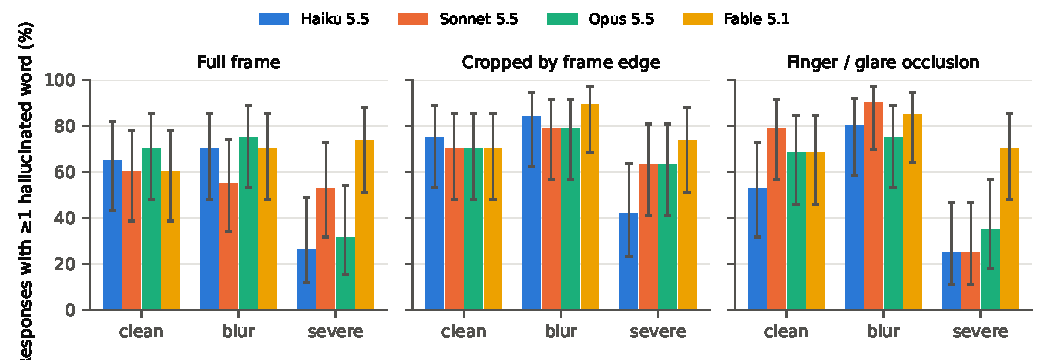
\includegraphics[width=\textwidth]{figures/fig_cells_real.pdf}
\caption{Study~2 (real images): share of description responses containing at least one hallucinated word, by image quality (x-axis) and framing (panels). Error bars are Wilson 95\% intervals; each bar is based on 19 or 20 images, so the intervals are wide and no cell contrast survives Holm correction (Section~\ref{sec:real}).}\label{fig:cells_real}
\end{figure}

\begin{figure}[t]
\centering
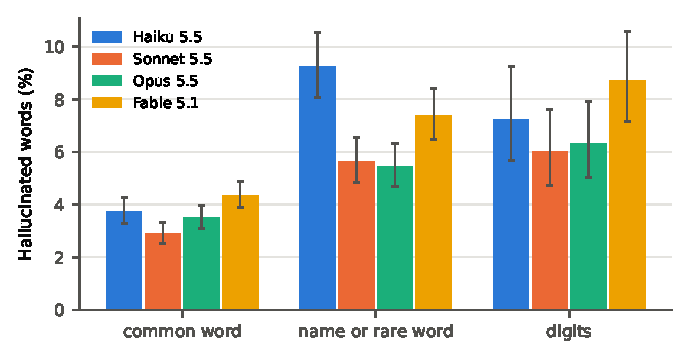
\includegraphics[width=0.72\textwidth]{figures/fig_categories_real.pdf}
\caption{Study~2: share of quoted words that are hallucinated, by the category of the ground-truth word they correspond to (description prompt). Error bars are Wilson 95\% intervals.}\label{fig:categories_real}
\end{figure}

\begin{figure}[t]
\centering
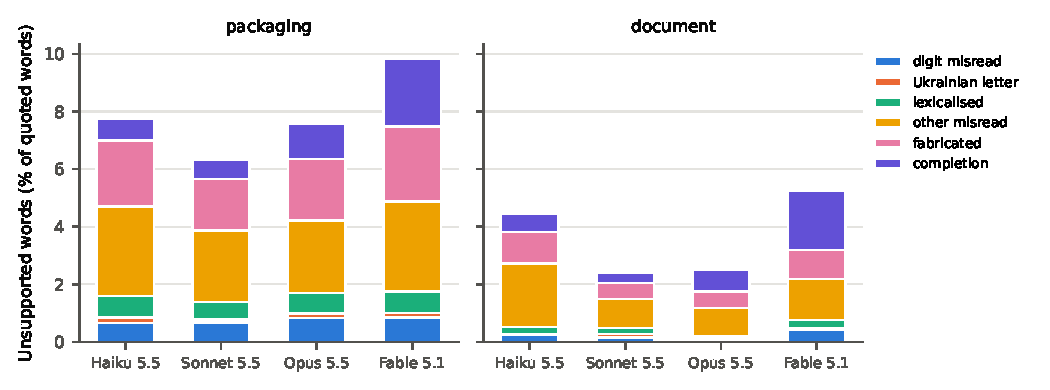
\includegraphics[width=\textwidth]{figures/fig_taxonomy_real.pdf}
\caption{Study~2: error taxonomy per model and genre, as a share of all quoted words in descriptions. ``Ukrainian letter'' marks substitutions of \foreignlanguage{ukrainian}{і, ї, є, ґ} by spellings shared with Russian; ``lexicalised'' marks a rare printed word reported as a common one. Rates are before the audit adjustment of Section~\ref{sec:audit_res}.}\label{fig:taxonomy_real}
\end{figure}

\begin{table}[t]
\caption{Study~2 (real packaging and documents, \RealNImages{} images): text-reading outcomes per model and prompt; columns as in Table~\ref{tab:rates}.}\label{tab:realrates}
\footnotesize
\setlength{\tabcolsep}{3pt}
\begin{tabular*}{\textwidth}{@{\extracolsep\fill}llrlrrrlr}
\toprule
Model & Prompt & Tokens & Hallucinated \% & Misread & Fabric. & Completion & Responses \% & Cover. \\
\midrule
%TABLE:realrates%
\botrule
\end{tabular*}
\end{table}

Detection transfers to real images with lower but still useful performance (Table~\ref{tab:realdetect}). The combined detector reaches AUROC \RealAucCombCIHaiku{} (Haiku), \RealAucCombCISonnet{} (Sonnet) and \RealAucCombCIOpus{} (Opus). At a 10\% false-flag rate it catches \RealRecTenHaiku\%, \RealRecTenSonnet\% and \RealRecTenOpus\% of hallucinated words. Cross-model agreement and OCR similarity remain the strongest single signals (Figure~\ref{fig:roc_real}).

\begin{figure}[t]
\centering
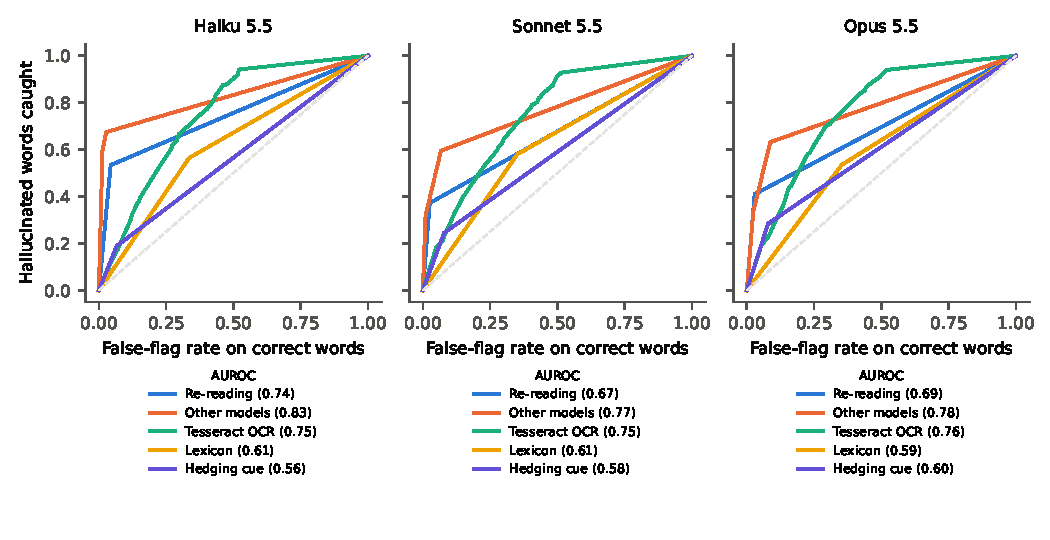
\includegraphics[width=\textwidth]{figures/fig_roc_real.pdf}
\caption{Study~2: ROC curves of the individual run-time signals for words quoted in descriptions of real images, per model. The legend gives each signal's AUROC.}\label{fig:roc_real}
\end{figure} Figure~\ref{fig:failures} shows four characteristic failures from the real-image runs.

\begin{table}[t]
\caption{Study~2: detection of hallucinated words in descriptions of real images; layout as in Table~\ref{tab:detect}.}\label{tab:realdetect}
\footnotesize
\begin{tabular*}{\textwidth}{@{\extracolsep\fill}lccc}
\toprule
Signal & Haiku 5.5 & Sonnet 5.5 & Opus 5.5 \\
\midrule
%TABLE:realdetect%
\botrule
\end{tabular*}
\end{table}

\begin{figure}[t]
\centering
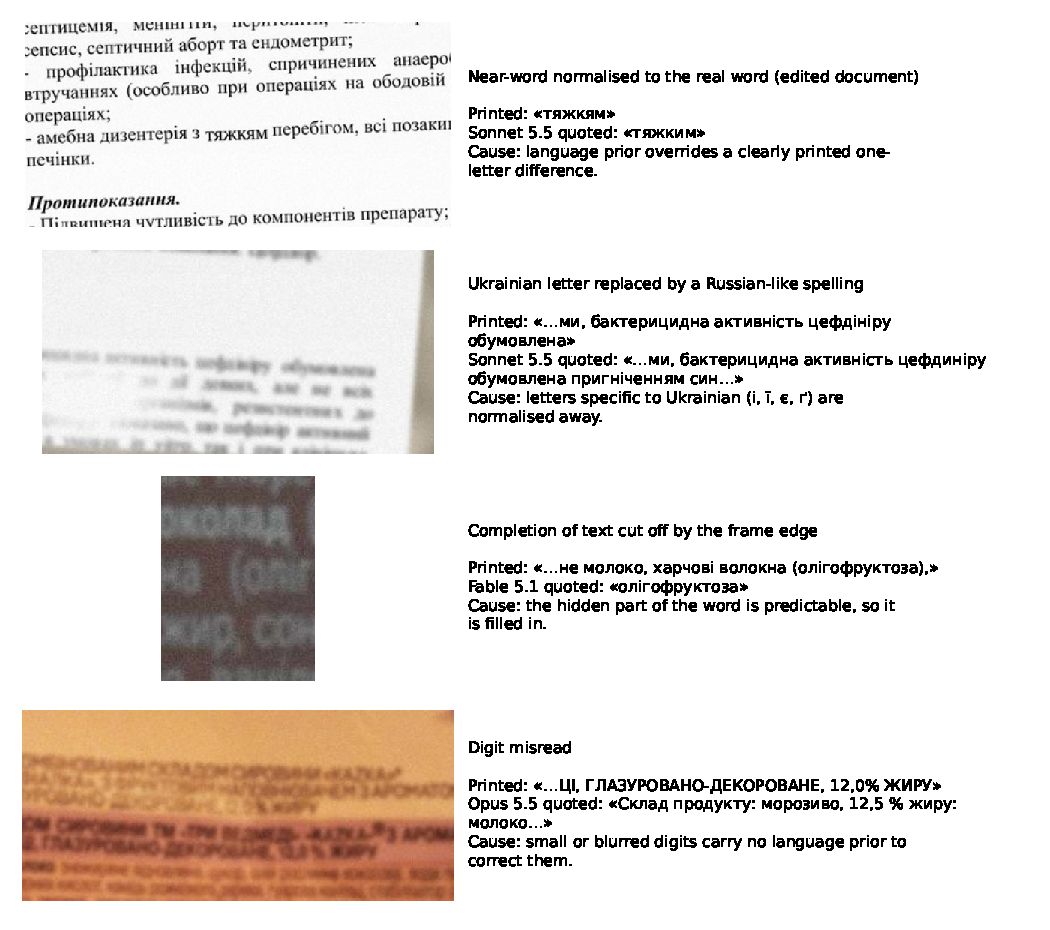
\includegraphics[width=\textwidth]{figures/fig_failures.pdf}
\caption{Failure cases from the real-image runs: crop of the stimulus around the token, printed text and quoted text. Top to bottom: a near-word on an edited medicine leaflet (probe, clean) reported as the real word; the Ukrainian spelling of a drug name (\foreignlanguage{ukrainian}{цефдініру}, leaflet of 3-Dinir, blur with glare) quoted in its Russian-like form; a word cut off by the frame edge (packaging, severe, crop) quoted in full; a fat content of ``12,0\% on an ice-cream label quoted as ``12,5\% (packaging, blur with glare). Cases were drawn with a fixed seed among Sonnet, Opus and Fable descriptions.}\label{fig:failures}
\end{figure}

\subsection{Near-word probe on real documents}\label{sec:probe_res}

On the \NProbePairs{} probe pairs, the four models quote the unedited real word correctly on \RangePrOrig\% of the original pages. On the edited pages they quote the printed near-word on only \RangePrNear\%, and on \RangePrNorm\% they quote the real word instead (Haiku \PrNormHaiku\%, Sonnet \PrNormSonnet\%, Opus \PrNormOpus\%, Fable \PrNormFable\%). For every model, the drop from reading the original correctly to reading the near-word correctly is significant (exact McNemar on the pairs: Haiku $p\PrPHaiku$, Sonnet $p\PrPSonnet$, Opus $p\PrPOpus$, Fable $p\PrPFable$). The edit is clearly visible at the probe's resolution (the target letters are at least 11~px high). Prior-driven normalisation is therefore not an artefact of synthetic rendering: on real official documents, the models report the word they expect (Figure~\ref{fig:probe}).

\begin{figure}[t]
\centering
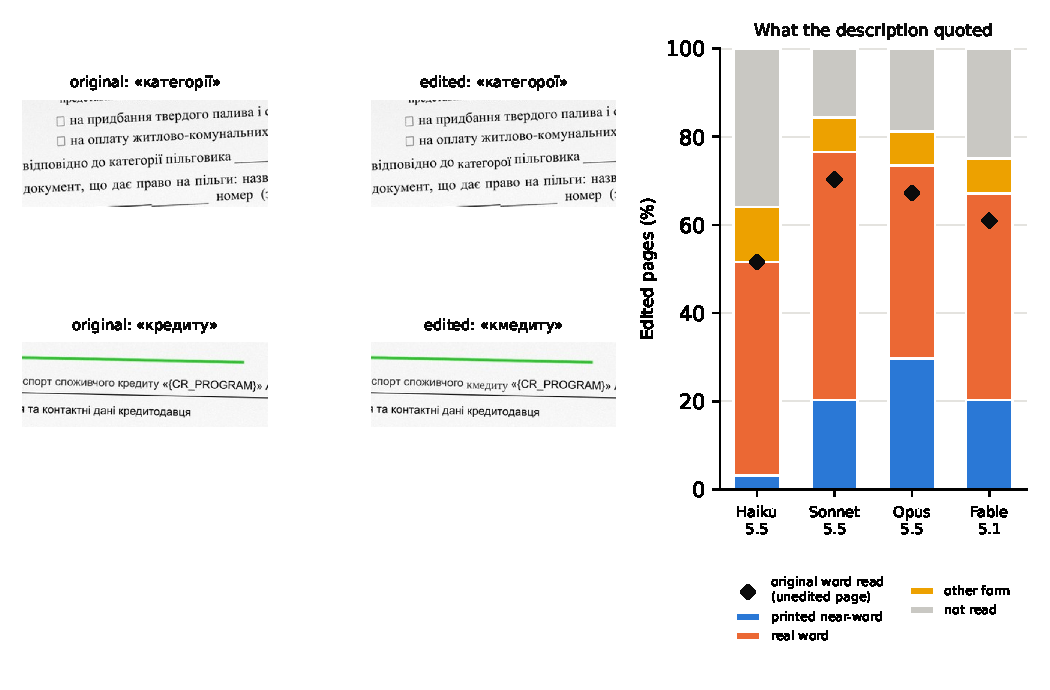
\includegraphics[width=\textwidth]{figures/fig_probe.pdf}
\caption{Near-word probe on real documents. Left: two of the \NProbePairs{} pairs (crop around the target on the original and the edited page, clean condition), drawn with a fixed seed among pages where at least three models reported the real word. Right: what each model's description quoted for the target on the edited pages, and how often it read the target correctly on the unedited original (diamonds).}\label{fig:probe}
\end{figure}

\subsection{Synthetic versus real stimuli}\label{sec:setcompare}

The two sets differ in ways that matter for interpretation. Real stimuli carry \RealTokPerImg{} ground-truth tokens per image against \SynTokPerImg{} in Study~1, with similar word length (mean \RealTokLen{} versus \SynTokLen{} letters). Names and rare words make up \RealNameShare\% of real tokens against \SynNameShare\% of synthetic ones, and digits \RealNumShare\% against \SynNumShare\%. Study~1 thus under-represents rare words and over-represents digits. The invented names of Study~1 over-represent the letters specific to Ukrainian relative to natural Ukrainian text (OpenSubtitles frequency list): \foreignlanguage{ukrainian}{ї} by a factor of \OverYi, \foreignlanguage{ukrainian}{є} by \OverYe{} and \foreignlanguage{ukrainian}{ґ} by \OverGhe. In the real texts, \foreignlanguage{ukrainian}{ґ} is almost absent (\RealGheShare\% of letters). The Ukrainian-letter error rate of Study~1 should therefore be read as a stress test, not as an estimate for everyday text. In Study~2, Ukrainian-letter substitutions make up only \RealSubUaHaiku\% (Haiku), \RealSubUaSonnet\% (Sonnet), \RealSubUaOpus\% (Opus) and \RealSubUaFable\% (Fable) of the hallucinated words, although they do occur on real leaflets (Figure~\ref{fig:failures}). Lexicalisations make up \RealRangeSubLex\% and fabrications \RealRangeSubFab\%. The main effects that Study~1 identified are reproduced on real images: hallucinated words in a majority of responses, unhedged errors, normalisation of near-words, degradation-driven misreading, and a usable combined detector. Their magnitudes differ.

\subsection{Run-to-run stability}\label{sec:stability}

The description prompt was run three times on \StabN{} Study~1 images, one per design cell (Table~\ref{tab:stab}). The image-level outcome (any hallucinated word) changes between runs for \StabFlipRange\% of the images. The token-level rate varies by at most \StabSpreadMax{} percentage points between runs. Point estimates of individual responses are therefore noisy, while the aggregate rates are stable. Disagreement between a model's own samples is a usable detector in its own right (AUROC \StabDisAucRange{} on this subset). This is comparable to, and for some models slightly above, the model's re-reading under the transcription prompt on the full set.

\begin{table}[t]
\caption{Run-to-run stability of the description prompt on \StabN{} Study~1 images (one per design cell), three runs per model. ``Flip'' is the share of images whose image-level outcome (any hallucinated word) is not the same in all three runs, with a Wilson 95\% interval. ``Disagr.'' is the AUROC of sample disagreement as a detector of hallucinated words in run~1.}\label{tab:stab}
\footnotesize
\begin{tabular*}{\textwidth}{@{\extracolsep\fill}lrlllrr}
\toprule
Model & Images & Any-hall.\ \% (r1/r2/r3) & Flip \% & Token rate \% (r1/r2/r3) & Spread & Disagr. \\
\midrule
%TABLE:stab%
\botrule
\end{tabular*}
\end{table}

\subsection{Automated audit of the labeller}\label{sec:audit_res}

On the Study~1 sample, the Claude rater confirms \SynAudCorrCl\% of correct labels, \SynAudMisCl\% of misreadings, \SynAudFabCl\% of fabrications and \SynAudComplCl\% of completions. On the Study~2 sample the corresponding figures are \RealAudCorrCl\%, \RealAudMisCl\%, \RealAudFabCl\% and \RealAudComplCl\%. Gemma~3 12B rated \SynAudNBoth{} of the Study~1 items before its server became unavailable. It confirms correct labels at a similar rate (\SynAudCorrGm\%) but judges most misread words to be printed as they were quoted (\SynAudMisGm\% confirmed). Inspection of its reasons shows that it does not resolve single-letter differences in Ukrainian words. Agreement between the raters on the printed-and-visible question is accordingly low (Cohen's $\kappa=\SynAudKappa$ on \SynAudNBoth{} items, raw agreement \SynAudAgree\%). Under the conservative resolution rule, \SynAudHall\% (\SynAudHallCI\%) of the Study~1 hallucination labels are confirmed. The Claude rater alone confirms \SynAudHallCl\%. For Study~2 the Claude rater confirms \RealAudHallCl\% of hallucination labels. The difference reflects reference gaps on real material, e.g., logos and stamps that are drawn as images rather than text and words that the reference OCR missed. Reported hallucination rates should therefore be read as upper bounds. Scaling the token-level rates of the descriptions by the Claude rater's confirmation rate gives audit-adjusted rates of \SynAdjRange\% for Study~1 and \RealAdjRange\% for Study~2. The large correction on real material is the main caveat on the Study~2 numbers. Gemma~3 was not available for the Study~2 sample, so these items have a single rater. One rater is a member of the evaluated family, and the other rater's own reading of Ukrainian is the bottleneck, so neither replaces a human validation.

\subsection{Cost and latency}\label{sec:cost}

Table~\ref{tab:cost} reports tokens, list-price cost and wall-clock time per image. All values were measured through the same command-line client, from the same machine and on the same days, so they are comparable across the four models but include client overhead and network time. On real images, a Haiku description costs \RealCostHaikuDesc{}~USD and takes about \RealCostHaikuDescSec{}~s. The re-reading call that the strongest single-model detector needs (a transcription by the same model) adds \RealCostHaikuTrans{}~USD and \RealCostHaikuTransSec{}~s for Haiku, and \RealCostOpusTrans{}~USD and \RealCostOpusTransSec{}~s for Opus. The cross-model signal requires two further descriptions, i.e., at least two to three times the cost and latency of a single description.

\begin{table}[t]
\caption{Cost and latency per image and call, by study, model and prompt: mean input tokens (including cached system-prompt tokens), mean output tokens, mean list-price cost in USD, and median (90th percentile) wall-clock seconds. All calls used the same command-line client path.}\label{tab:cost}
\footnotesize
\setlength{\tabcolsep}{3pt}
\begin{tabular*}{\textwidth}{@{\extracolsep\fill}lllrrrrr}
\toprule
Study & Model & Prompt & Calls & In tok. & Out tok. & USD & Seconds \\
\midrule
%TABLE:cost%
\botrule
\end{tabular*}
\end{table}

\begin{table}[t]
\caption{Pairwise model comparisons on shared images (description prompt). ``Any-hall.'' gives the share of images with at least one hallucinated word for the first / second model; ``Disc.'' the discordant pairs (first only / second only); $p$ is the exact McNemar test, Holm-corrected across the six pairs of each study; the last column is the difference in token-level hallucination rate (first minus second, percentage points) with a paired cluster-bootstrap 95\% interval.}\label{tab:pairs}
\footnotesize
\setlength{\tabcolsep}{3pt}
\begin{tabular*}{\textwidth}{@{\extracolsep\fill}lrrrrl}
\toprule
Pair & Images & Any-hall.\ \% & Disc. & $p_\mathrm{Holm}$ & $\Delta$ token rate [95\% CI] \\
\midrule
%TABLE:pairs%
\botrule
\end{tabular*}
\end{table}
